\chapter{Tutorial}
\label{cha:tutorial}

This chapter discusses the \fun{dynopt} application. It shows, that
\fun{dynopt} is suitable for a quite large variety of problems
ranging from simple unconstrained problem to inequality state path
constraint problem described either by ODE's or DAE's. As mentioned in
the title of this chapter, it is an step by step tutorial. It shows
the user how to define his problem into \fun{dynopt} by filling the
input argument functions \fun{process}, \fun{objfun}, \fun{confun}. 

\section{ODE systems}
\label{sec:odes}

\subsection{Example 1: Unconstrained Problem}
\label{sec:unconprob}

Consider a simple integrator with LQ cost function to be
optimised \citep{luu91,raj01} (MATLAB code for this example is located
at \subor{examples/problem1a}): 
\begin{gather}
\dot{x}_1 = u, \quad x_{1}(0) = 1\\
\dot{x}_2 = x^{2}_{1} + u^{2}, \quad x_{2}(0) = 0
\end{gather}
The cost function is given in the Mayer form:
\begin{equation}
\min_{\ve{u}(t)} \mf{J} = x_{2}(t_{f}) \label{eq:ucp} 
\end{equation} with $x_{1}(t),~x_{2}(t)$ as states and $u(t)$ as
control, such that $t_{f} = 1$.

\subsubsection{Function~\fun{process},~\fun{objfun}  definitions}
\label{sec:unconprob-fundef}

Problem \eqref{eq:ucp} is described by two differential equations
which together with initial values of state variables should be
defined in \fun{process}.

\paragraph{Step1: Write an M-file~\subor{process.m}}

{\small \verbatiminput{examples/problem1a/process.m}}

It is important to notice that in \fun{dynopt} the mass matrix
$\ve{M}$ \eqref{eq:process} is by default a $nx$-by-$nx$ identity
matrix. Here $nx$ represents the number of state variables $x$. 

As the performance index is given in Mayer form, \fun{dynopt} 
optimises it at final conditions, thus the input arguments of
\fun{objfun} are as follows: \argfun{t}~-~scalar value $t_{f}$,
\argfun{x}~-~scalar/vector of state variable(s),
\argfun{u}~-~scalar/vector of control variable(s), both evaluated at
corresponding  final time $t_{f}$, \argfun{p}~-~scalar/vector of time
independent parameters. \fun{objfun} should be defined as follows:

\paragraph{Step2: Write an M-file~\subor{objfun.m}}

{\small \verbatiminput{examples/problem1a/objfun.m}}

After the problem has been defined in the functions, user has to invoke
the \fun{dynopt} function by writing an M-file \subor{problem1a.m} as
follows:

\paragraph{Step3: Invoke~\fun{dynopt}}

{\small \verbatiminput{examples/problem1a/problem1a.m}}

In this case the variables: \argfun{t}, \argfun{u} were chosen as
decision variables, so the parameter \argfun{optimparam.optvar} was
set to 3. As the objective is to minimise the functional in Mayer form
the parameter \argfun{optimparam.objtype} was left an empty
matrix. Moreover 3 collocation points for state variables
(\argfun{optimparam.ncolx}), 2 collocation points for control
variables (\argfun{optimparam.ncolu}), 3 time intervals with the same
initial lengths (\argfun{optimparam.li}) equal to $1/3$ were
chosen. Final time $t_f = 1$ was given by the problem definition
(\argfun{optimparam.tf}), the control variable initial values
(\argfun{optimparam.ui}) were set to 0 for each time interval. As can
be seen from the problem definition \eqref{eq:ucp} no parameters
(\argfun{optimparam.par}), no bounds for the control variables 
(\argfun{optimparam.bdu}), the state variables (\argfun{optimparam.bdx}),
and the parameters (\argfun{optimparam.bdp}) are needed, so the values
of this parameters have been left an empty matrix. As mentioned before,
this problem is unconstrained, so parameter \argfun{optimparam.confun}
was set to [~].

The results returned by \fun{dynopt} in \argfun{optimout} structure
contain the vector of times \argfun{t}, the vector of optimal control
profile \argfun{u}. They are ready to be plotted.\\
The objective function at the optimal solution [\argfun{t},\argfun{u}]
is returned after 133 iterations in above mentioned output structure
\argfun{optimout} as parameter \argfun{fval}:
\begin{verbatim}
optimout.fval = 7.615959e-01
\end{verbatim}
The parameter \argfun{exitflag} tells if the algorithm converged. An
\argfun{exitflag} $>$ 0 means a local minimum was found: 
\begin{verbatim}
optimout.exitflag = 1
\end{verbatim}
More details about the optimisation are given by the
\argfun{optimout.output} structure. In this example, the default
selection of the large-scale algorithm has been turned off, so the
medium-scale algorithm is used. Also all termination tolerances have
been changed. For more information about \argfun{options} and
\fun{dynopt} input and output arguments, see Chapter~\ref{cha:reference}. 

The user may want to plot also the state profiles but without
integrating the \fun{process} with respect to the optimal control
profile in \argfun{optimout.u}. It is possible to use an additional
function \fun{profiles} for this reason as follows:
\begin{verbatim}
[tplot,uplot,xplot] = profiles(optimout,optimparam,ntimes);
\end{verbatim}
where \argfun{ntimes} represents the density of the points plotted per
interval. Note that profiles are represented by collocation
polynomials and not as a solution of the original ODE/DAE
system. Therefore, there might be slight differences with regard to
the original problem. For more precise plots, integrate the original
problem with optimal control trajectories.

Graphical representation of the problem \eqref{eq:ucp} solution is
shown in Figs.~\ref{fig:prob1a_u_323n} and \ref{fig:prob1a_x12_323n}. 

\begin{figure}[htb]
\begin{minipage}[t]{0.5\linewidth}
\centering
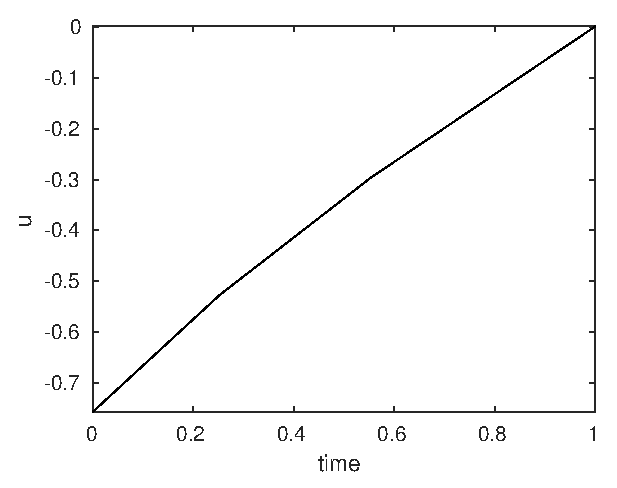
\includegraphics[width=0.99\textwidth]{examples/problem1a/graphs/u_323n.eps}
\caption[Tutorial example 1: control profile]{Control profile for
  unconstrained problem} \label{fig:prob1a_u_323n} 
\end{minipage}
\begin{minipage}[t]{0.5\linewidth}
\centering
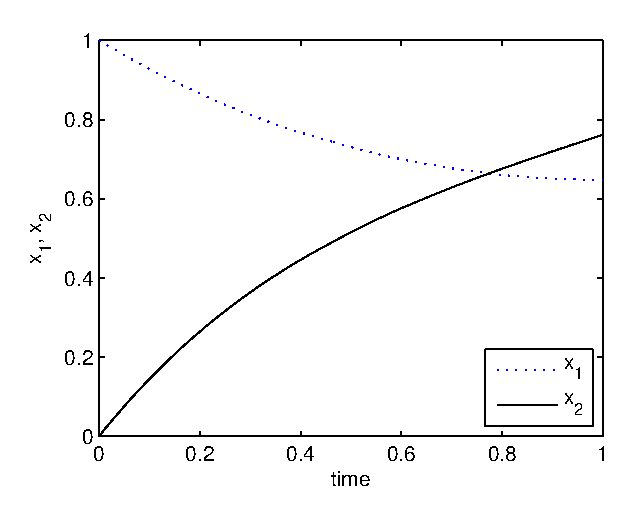
\includegraphics[width=0.99\textwidth]{examples/problem1a/graphs/x12_323n.eps}
\caption[Tutorial example 1: state profiles]{State profiles for
  unconstrained problem} \label{fig:prob1a_x12_323n} 
\end{minipage}
\end{figure}

\subsection{Example 2: Constrained Problem with Gradients}
\label{sec:conprobgrad}

A process described by the following system of 2
ODE's \citep{raj01,luu91} (MATLAB code for this example is located
at \subor{examples/problem1b}):   
\begin{gather}
\dot{x}_1 = u, \quad x_{1}(0) = 1\\
\dot{x}_2 = x^{2}_{1} + u^{2}, \quad x_{2}(0) = 0
\end{gather} is to be optimised for $u(t)$ with the cost function:
\begin{equation}
\min_{\ve{u}(t)} \mf{J} = x_{2}(t_{f}) \label{eq:cpg} 
\end{equation} subject to the constraint:
\begin{equation}
x_{1}(1) = 1
\end{equation} with $x_{1}(t),~x_{2}(t)$ as states, $u(t)$ as control,
such that $t_{f} = 1$. 

Problem \eqref{eq:ucp} is similar to problem \eqref{eq:cpg}, it 
differs in constraint of state variable $x_{1}$ at final time
$t_{f}=1$. This example will be solved by supplying analytical
gradients. Ordinarily the medium-scale minimisation routines use
numerical gradients calculated by finite-difference
approximation. This procedure systematically perturbs each of the
variables in order to calculate function and constraint partial
derivatives. Alternatively, you can provide a function to compute 
partial derivatives analytically. Typically, the problem is solved
more accurately and efficiently if such a function is provided. 

\subsubsection{Function~\fun{process},~\fun{objfun},~\fun{confun}  definitions}
\label{sec:conprobgrad-fundef}

As mentioned before the problem \eqref{eq:cpg} is described by the
same differential equations as problem \eqref{eq:ucp}. As we decided
to supply analytical gradients, they should be defined for all the
user supplied functions: \fun{process}, \fun{objfun},
\fun{confun}. The form of the gradients will be explained on the
function \fun{process} and is valid for all above mentioned user
functions.  

\paragraph{Step1: Write an M-file~\subor{process.m}}

{\small \verbatiminput{examples/problem1b/process.m}}

Definition of gradients results from problem definition
\eqref{eq:cpg}. As the problem consists of one control variable $u$
and two states variables $x_{1}, x_{2}$ just the gradients with
respect to this variables have to be supplied by filling the
appropriate flag.\\ 
\argfun{sys} in case 1 contains the partial derivatives of the
\fun{process} function, defined as \argfun{sys} in case 0, with
respect to each of the elements in \argfun{x}: 
\begin{displaymath}
\argfun{sys} = 
\begin{bmatrix}
\frac{\displaystyle \partial{f_{1}}}{\displaystyle \partial{x_{1}}} &
\frac{\displaystyle \partial{f_{2}}}{\displaystyle \partial{x_{1}}}\\
\frac{\displaystyle \partial{f_{1}}}{\displaystyle \partial{x_{2}}} &
\frac{\displaystyle \partial{f_{2}}}{\displaystyle \partial{x_{2}}}
\end{bmatrix} =
\begin{bmatrix}
0 & 2x_{1}\\
0 & 0
\end{bmatrix}
\end{displaymath}
\argfun{sys} in case 2 contains the partial derivatives of the
\fun{process} function, defined as \argfun{sys} in case 0, with
respect to each of the elements in \argfun{u}:
\begin{displaymath}
\argfun{sys} = 
\begin{bmatrix}
\frac{\displaystyle \partial{f_{1}}}{\displaystyle \partial{u}} &
\frac{\displaystyle \partial{f_{2}}}{\displaystyle \partial{u}}
\end{bmatrix} =
\begin{bmatrix}
1 & 2u
\end{bmatrix} 
\end{displaymath}
If needed, the gradients with respect to other defined variables
(\argfun{t}, \argfun{p}) are filled similarly. For more information
about \fun{process} definition, and its input and output arguments
see chapter \ref{cha:reference}.

As mentioned before user has also to supply the gradients to the
objective function \fun{objfun} as follows: 

\paragraph{Step2: Write an M-file~\subor{objfun.m}}

{\small \verbatiminput{examples/problem1b/objfun.m}}

Here they are written in the structure \argfun{Df} containing
variables \argfun{t}, \argfun{u}, \argfun{x}, and \argfun{p} and
representing the gradients with respect to the appropriate
variable. Just the variables used in problem are filled by
user. Unused variables are set to be an empty matrix. For more
information about \fun{objfun} definition, and its input and output
arguments see chapter \ref{cha:reference}. 

\fun{dynopt} optimises a given performance index, subject to the
constraints defined at the beginning $t =
t_{0}$ (\argfun{flag} = 0), over the full time interval $t \in
[t_{0},t_{f}]$ (\argfun{flag} = 1), and at the end $t = t_{f}$
(\argfun{flag} = 2). Thus the input arguments of \fun{confun} are the
same as of \fun{process} but it is necessary to tell \fun{dynopt} by
defining the constraints and their gradients with respect to the
appropriate variables in the corresponding flag in which time should
they be evaluated. How the gradients have to seem like, was explained
before. \fun{confun} should be defined as follows:  
 
\paragraph{Step3: Write an M-file~\subor{confun.m}}

{\small \verbatiminput{examples/problem1b/confun.m}}

Here the gradients are written into the structures \argfun{Dc},
\argfun{Dceq} similar to those, described in \fun{objfun}. For more
information about \fun{confun} definition, and its input and output
arguments see chapter \ref{cha:reference}.

Since you are providing the gradients of the objective function in
\subor{objfun.m} and the gradients of the constraints in
\subor{confun.m}, you must tell \fun{dynopt} that these M-files
contain this additional information. Use optimset to turn the
parameters \argfun{GradObj} and \argfun{GradConstr} to 'on' in our
already existing options structure 
\begin{verbatim}
options = optimset(options,'GradObj','on','GradConstr','on');
\end{verbatim}
If you do not set these parameters to 'on' in the options structure,
\fun{dynopt} will not use the analytic gradients.  

After the problem has been defined in the functions, user has to invoke
the \fun{dynopt} function by writing an M-file \subor{problem1b.m} as
follows :

\paragraph{Step4: Invoke~\fun{dynopt}}

{\small \verbatiminput{examples/problem1b/problem1b.m}}

As this problem differs from the problem \eqref{eq:ucp} in the
constraint applied in final time $t_{f} = 1$, the input parameter
\argfun{optimparam.confun} is set to the constraint function name
$@confun$. Next, 3 collocation points for state variables, 2 intervals
with the same initial lengths of intervals equal to $1/2$ have been
chosen. Other parameters are as same as in problem \eqref{eq:ucp}.

The optimal solution is shown in Figs. \ref{fig:prob1b_u} and
\ref{fig:prob1b_x}. The value of the objective function at this
solution is 9.242532e-01 after 45 iterations and with \argfun{exitflag}
equal to~2.

\begin{figure}[htb]
\begin{minipage}[t]{0.5\linewidth}
\centering
\includegraphics[width=0.99\textwidth]{examples/problem1b/graphs/u_624a.eps}
\caption[Tutorial example 2: control profile]{Control profile for
  constrained problem with gradients} \label{fig:prob1b_u} 
\end{minipage}
\begin{minipage}[t]{0.5\linewidth}
\centering
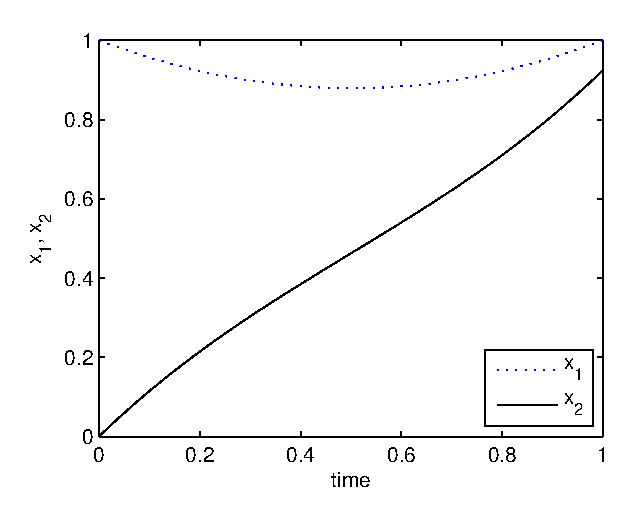
\includegraphics[width=0.99\textwidth]{examples/problem1b/graphs/x12_624a.eps}
\caption[Tutorial example 2: state profiles]{State profiles for
  constrained problem with gradients} \label{fig:prob1b_x} 
\end{minipage}
\end{figure}

Alternative NLP solver Ipopt can be invoked when uncommenting the line 
\begin{verbatim}
options.NLPsolver='ipopt';
\end{verbatim}
in the main file. A~slightly better value of the optimum is found in
8047 iterations and the value of the objective function is
9.2423977e-01. More about alternate NLP solvers can be found in
Chapter~\ref{cha:reference}.

\subsection{Example 3: Unconstrained Problem  with Gradients and Bounds}
\label{sec:unconprobgradbound}

Following mathematical problem \citep{raj01,luu90_51} with system of
four ODE's (MATLAB code for this example is located at
\subor{examples/problem2}):
\begin{gather}
\dot{x}_1 = x_{2}, \quad x_{1}(0) = 0\\
\dot{x}_2 = -x_{3}u + 16t - 8, \quad x_{2}(0) = -1\\
\dot{x}_3 = u, \quad x_{3}(0) = -\sqrt{5}\\
\dot{x}_4 = x_{1}^{2} + x_{2}^{2} + 0.0005(x_{2} + 16t - 8 -
0.1x_{3}u^{2})^{2}, \quad x_{4}(0) = 0
\end{gather} is to be optimised for $-4 \leq u(t) \leq 10$ with the
cost function:  
\begin{equation}
\min_{\ve{u}(t)} \mf{J} = x_{4}(t_{f}) \label{eq:ucpgb}
\end{equation} with $x_1(t) - x_4(t)$ as states, $u(t)$ as control,
such that $t_{f}=1$. 

\subsubsection{Function~\fun{process},~\fun{objfun},~\fun{confun}  definitions}
\label{sec:unconprbgradbound-fundef}

\paragraph{Step1: Write an M-file~\subor{process.m}}

{\small \verbatiminput{examples/problem2/process.m}}

\paragraph{Step2: Write an M-file~\subor{objfun}}

{\small \verbatiminput{examples/problem2/objfun.m}}

\paragraph{Step3: Invoke~\fun{dynopt}} writing an M-file
\subor{problem2.m} as follows: 

{\small \verbatiminput{examples/problem2/problem2.m}}

The value of the objective function evaluated for optimal control
profile is of value of 1.202688e-01 after 175 iterations with exitflag
equal to~1 (using default NLP solver~\fun{fmincon}). Graphical
representation of the solution of the problem \eqref{eq:ucpgb} is
shown in Figs. \ref{fig:prob2_u} and \ref{fig:prob2_x}. Ipopt solver
finished after 2565 iterations with the cost function value of
1.2047839e-01. 

\begin{figure}[htb]
\begin{minipage}[t]{0.5\linewidth}
\centering
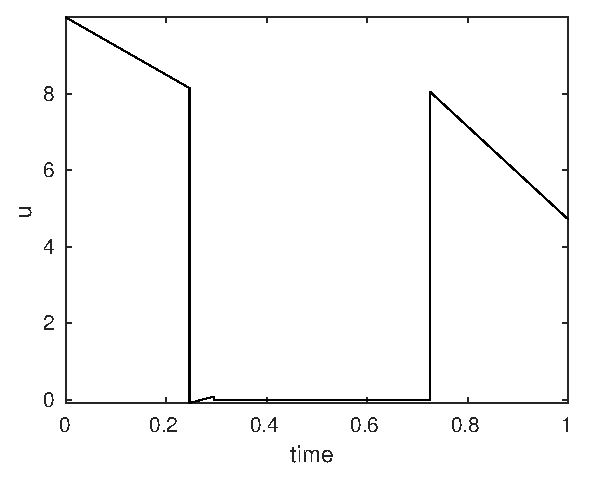
\includegraphics[width=0.99\textwidth]{examples/problem2/graphs/u_624a.eps}
\caption[Tutorial example 3: control profile]{Control profile for
  unconstrained problem with gradients and bounds} \label{fig:prob2_u} 
\end{minipage}
\begin{minipage}[t]{0.5\linewidth}
\centering
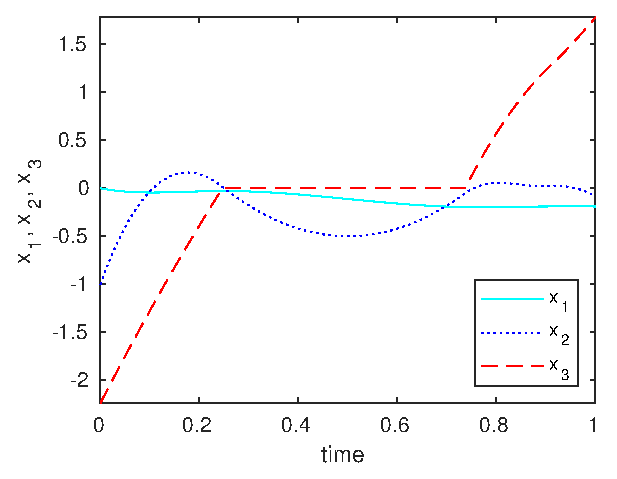
\includegraphics[width=0.99\textwidth]{examples/problem2/graphs/x13_624a.eps}
\caption[Tutorial example 3: state profiles]{State profiles for
  unconstrained problem with gradients and bounds} \label{fig:prob2_x}
\end{minipage}
\end{figure}

\subsubsection{Control Constrained on Intervals}
If we would like to constrain control on the first interval to be at
most 9, we will redefine variable \argfun{bdu}
(\subor{examples/problem2_bdu/problem2bdu.m}).  Now it will be a matrix composed
of lower and upper bounds on every interval as follows
\begin{verbatim}
optimparam.bdu = [-4 9 -4 10 -4 10 -4 10]; 
\end{verbatim}

The value of the objective function evaluated for optimal control
profile has increased to 0.1249686 after 154 iterations with exitflag
equal to~1. Graphical representation of the modified solution is shown
in Figs. \ref{fig:prob2bdu_u} and \ref{fig:prob2bdu_x}.

\begin{figure}[htb]
\begin{minipage}[t]{0.5\linewidth}
\centering
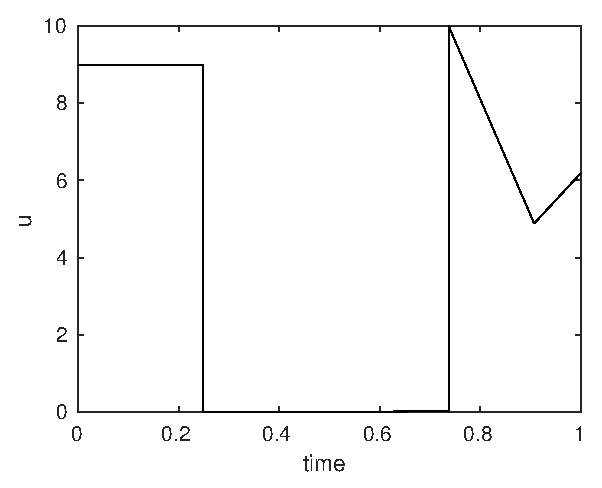
\includegraphics[width=0.99\textwidth]{examples/problem2_bdu/graphs/u_624bdu.eps}
\caption[Tutorial example 3: control profile]{Control profile for
  unconstrained problem with gradients and bounds on intervals} \label{fig:prob2bdu_u} 
\end{minipage}
\begin{minipage}[t]{0.5\linewidth}
\centering
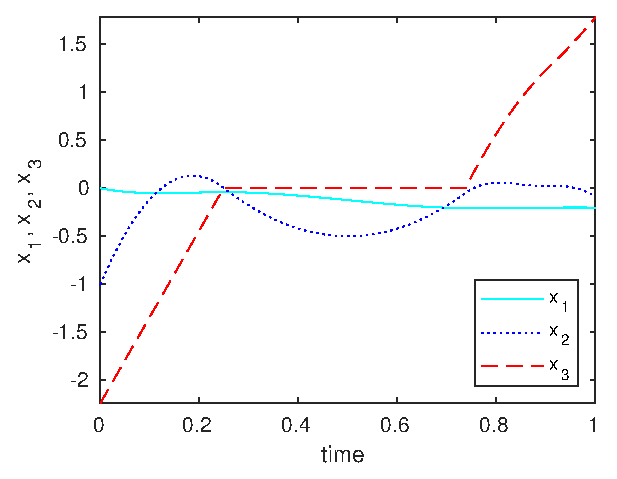
\includegraphics[width=0.99\textwidth]{examples/problem2_bdu/graphs/x13_624bdu.eps}
\caption[Tutorial example 3: state profiles]{State profiles for
  unconstrained problem with gradients and bounds on intervals} \label{fig:prob2bdu_x}
\end{minipage}
\end{figure}

\subsection{Example 4: Inequality State Path Constraint Problem}
\label{sec:statepathconprob}

A~process described by the following system of 2
ODE's \citep{jac69,fee98} (MATLAB code for this example is located
at \subor{examples/problem3}):
\begin{align}
\dot{x}_1 &= x_{2}, &\quad x_{1}(0) &= 0\\
\dot{x}_2 &= -x_{2} + u, &\quad x_{2}(0) &= -1
\end{align}is to be optimised for $u(t)$ with the cost function:
\begin{equation}
\min_{\ve{u}(t)} \mf{J} = \int_{0}^{1}(x_{1}^{2} + x_{2}^{2} +
0.005u^{2})\dt \label{eq:ispcpa} 
\end{equation} subject to state path constraint:
\begin{equation}
x_{2} - 8(t - 0.5)^{2} + 0.5 \leq 0, \quad t \in [0,1]  
\end{equation} with $x_{1}(t),~x_{2}(t)$ as states, $u(t)$ as control,
such that $t_{f}=1$. 

As the objective function is not in the Mayer form as required by
\fun{dynopt}, we define an additional differential equation
\begin{equation}
\dot{x}_3 =  x_1^2+x_2^2+0.005u^2, \quad x_3(0) = 0
\end{equation}
and rewrite the cost as
\begin{equation} 
\min_{\ve{u}(t)} \mf{J} = x_3(t_f) \label{eq:ispcpb} 
\end{equation}

\subsubsection{Function~\fun{process},~\fun{objfun},~\fun{confun}  definitions}
\label{sec:statepathconprob-fundef}

\paragraph{Step1: Write an M-file \subor{process.m}}

{\small \verbatiminput{examples/problem3/process.m}}

\paragraph{Step2: Write an M-file~\subor{objfun}}

{\small \verbatiminput{examples/problem3/objfun.m}}

\paragraph{Step3: Write an M-file~\subor{confun}}

{\small \verbatiminput{examples/problem3/confun.m}}

\paragraph{Step4: Invoke~\fun{dynopt}} writing an
M-file~\subor{problem3.m} as follows: 

{\small \verbatiminput{examples/problem3/problem3.m}}

An optimal value of $x_{3}(t_{f})=0.1701564$ was computed after 3342
iterations with exitflag equal to~1 (using~\fun{fmincon}). Graphical
representation of the solution of the problem~\eqref{eq:ispcpb} is
shown in Figs. \ref{fig:prob3_u}, \ref{fig:prob3_x}, and
\ref{fig:prob3_c}.

\begin{figure}[htb]
\begin{minipage}[t]{0.5\linewidth}
\centering
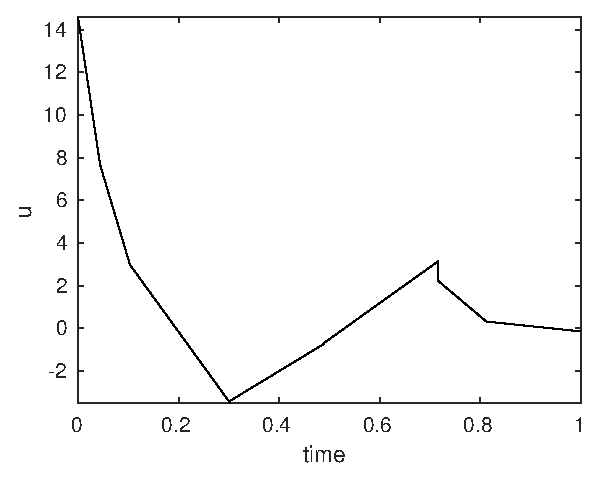
\includegraphics[width=0.99\textwidth]{examples/problem3/graphs/u_627a.eps}
\caption[Tutorial example 4: control profile]{Control profile for
  inequality state path constraint problem} \label{fig:prob3_u}
\end{minipage}
\begin{minipage}[t]{0.5\linewidth}
\centering
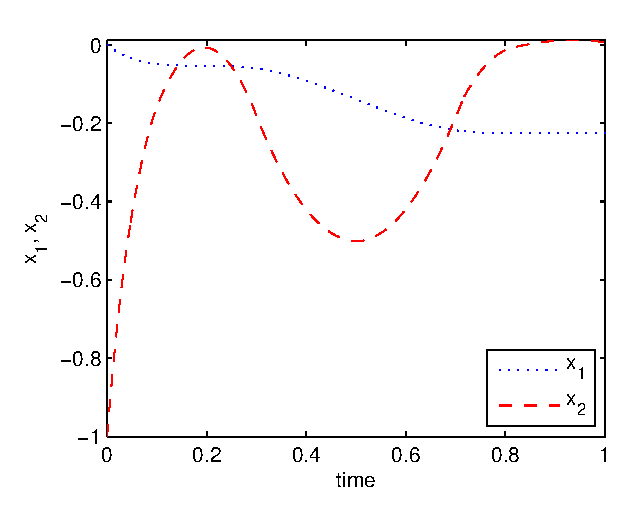
\includegraphics[width=0.99\textwidth,clip]{examples/problem3/graphs/x12_627a.eps}
\caption[Tutorial example 4: state profiles]{State profiles for
  inequality state path constraint problem} \label{fig:prob3_x}
\end{minipage}
\begin{minipage}[t]{0.5\linewidth}
\centering
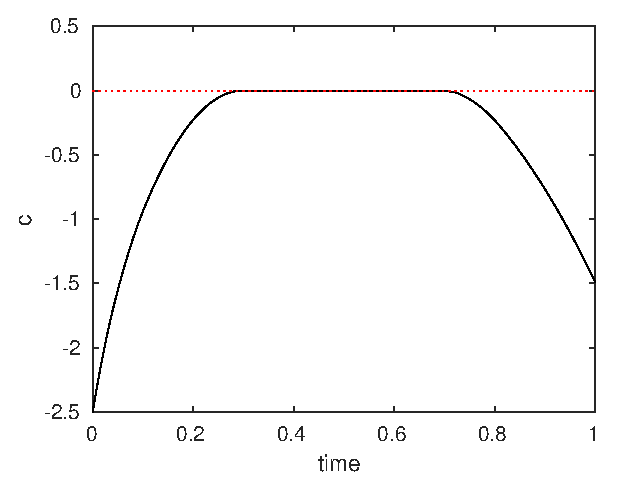
\includegraphics[width=0.99\textwidth,clip]{examples/problem3/graphs/c_627a.eps}
\caption[Tutorial example 4: constraints]{Constraint profile for
  inequality state path constraint problem} \label{fig:prob3_c}
\end{minipage}
\begin{minipage}[t]{0.5\linewidth}
\centering
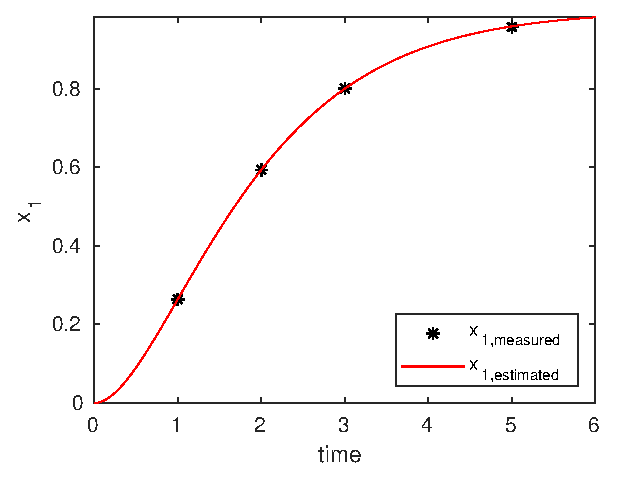
\includegraphics[width=0.99\textwidth,clip]{examples/problem8/graphs/xpa.eps}
\caption[Tutorial example 5: state profiles]{Comparison of estimated
  and measured state trajectory for state $x_{1}$ in parameter
  estimation problem} \label{fig:prob8_x} 
\end{minipage}
\end{figure}

\subsection{Example 5: Parameter Estimation Problem}
\label{sec:pep}

Consider a state estimation problem~\cite{fik02} where the cost
functional is defined as the sum of squares of deviations between the
model and measured outputs as follows (MATLAB code for this example is
located at \subor{examples/problem8}):
\begin{equation}
\min_{\ve{p}} \mf{J} =
\sum_{i=1,2,3,5}(x_{1}(t_{i})-x_{1}^{\text{m}}(t_{i}))^{2}
\label{eq:pep}  
\end{equation}
subject to the following ODE's:
\begin{align}
\dot{x}_{1} &= x_{2}, &\qquad x_{1}(0) &= p_{1} \\
\dot{x}_{2} &= 1 - 2x_{2} - x_{1}, &\qquad x_{2}(0) &= p_{2}
\end{align} with $x_{1}, x_{2}$ as states and $t_f = 6$.
The task is to find initial conditions denoted by the parameters
$p_{1}, p_{2} \in [-1.5,1.5]$, if the input to the system is equal to
1. Measured outputs $x_{1}^{\text{m}}$ and times of measurements are
specified in Tab.~\ref{tab:measureddatas}.  

\begin{table}[h]
  \begin{center}
    \begin{tabular}{|c|c|c|c|c|}
      \hline
      $t$ & 1 & 2 & 3 & 5\\
      $x_{1}^{\text{m}}$ & 0.264 & 0.594 & 0.801 & 0.959\\
      \hline
    \end{tabular}
  \end{center}
  \caption{Measured data for parameter estimation problem}
  \label{tab:measureddatas} 
\end{table}
 
\subsubsection{Function~\fun{process},~\fun{objfun},~\fun{confun}  definitions}

\paragraph{Step1: Write an M-file \subor{process.m}}

{\small \verbatiminput{examples/problem8/process.m}}

\paragraph{Step2: Write an M-file~\subor{objfun}}

{\small \verbatiminput{examples/problem8/objfun.m}}

\paragraph{Step3: Write an M-file~\subor{confun}}

{\small \verbatiminput{examples/problem8/confun.m}}

\paragraph{Step4: Invoke~\fun{dynopt}} writing an
M-file~\subor{problem8.m} as follows:

{\small \verbatiminput{examples/problem8/problem8.m}}

The results obtained by \fun{dynopt} are the same as those published
in \cite{fik02}. Fig. \ref{fig:prob8_x} shows the comparison of
estimated and measured state trajectory. 

\subsection{Example: Minimum Time Problem}
\label{sec:car}

Consider a following problem optimising a car that has to be moved
from origin and stopped at a distance of 300\,m in a minimum time
(MATLAB code for this example is located at
\subor{examples/problem-car})
\begin{align}
\dot{x}_1 &= u, \quad  &x_{1}(0) &= 0 , \quad  &x_{1}(t_f) &= 0 \\
\dot{x}_2 &= x_{1}, \quad &x_{2}(0) &= 0, \quad  &x_{2}(t_f) &= 300  
\end{align} 
optimised for $-2 \leq u(t) \leq 1$ with the cost function:
\begin{equation} \label{eq:car}
\min_{u(t)} \mf{J} = t_{f} 
\end{equation} 
with $x_1(t)$ -- velocity, $x_2(t)$ -- distance, $u(t)$ control --
acceleration.

\subsubsection{Function~\fun{process},~\fun{objfun},~\fun{confun}  definitions}
\label{sec:car-fundef}

\paragraph{Step1: Write an M-file~\subor{process.m}}

{\small \verbatiminput{examples/problem-car/process.m}}

\paragraph{Step2: Write an M-file~\subor{objfun}}

{\small \verbatiminput{examples/problem-car/objfun.m}}

\paragraph{Step3: Invoke~\fun{dynopt}} writing an M-file
\subor{car.m} as follows. Note that optimising the final time is
indicated by setting it to an empty matrix: \verb+optimparam.tf=[]+
and by optimising the time interval lengths. 

{\small \verbatiminput{examples/problem-car/car.m}}

The value of the objective function evaluated for optimal control
profile is of value of 30.00 after 85 iterations with exitflag equal
to~1 (\fun{fmincon}) or after 28 iterations (\fun{ipopt}). Graphical
representation of the solution of the problem~\eqref{eq:car} is shown
in Fig.~\ref{fig:car}.

\begin{figure}[htb]
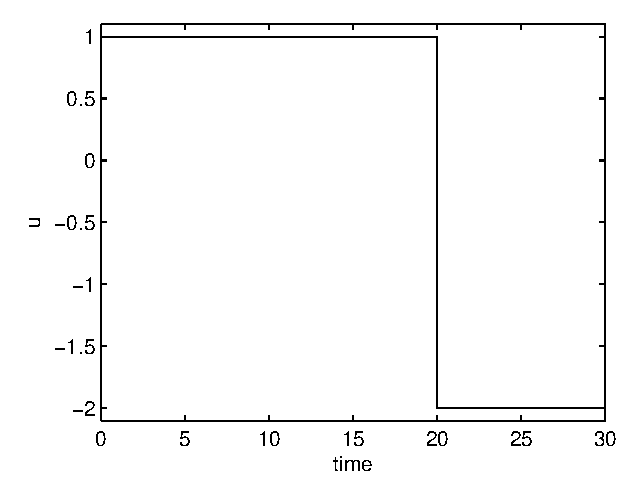
\includegraphics[width=0.49\textwidth]{examples/problem-car/car_u.eps}
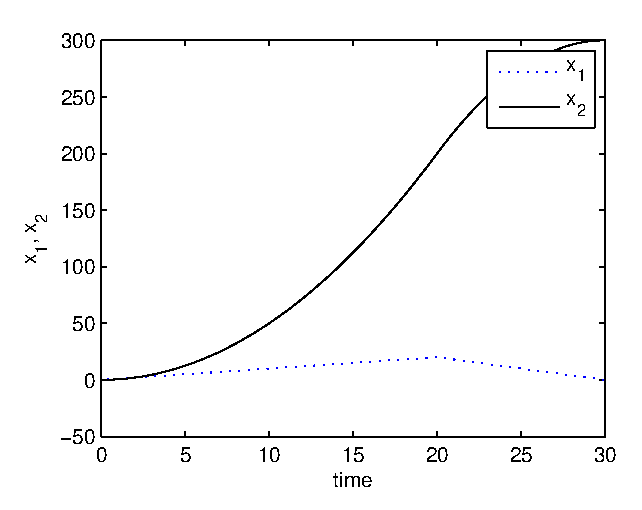
\includegraphics[width=0.49\textwidth]{examples/problem-car/car_x.eps}
\caption{Control and state profiles for minimum time car
  problem} \label{fig:car}
\end{figure}

The same problem with constrained velocity during the whole trajectory
$x_1 < 10$ (MATLAB code for this example is located at
\subor{examples/problem-car2}) converged to the minimum value of 37.50
after 139/31 iterations (fmincon/ipopt). Graphical representation of
the solution is shown in Fig.~\ref{fig:car2}.


\begin{figure}[htb]
\includegraphics[width=0.32\textwidth]{examples/problem-car2/car_u.eps}
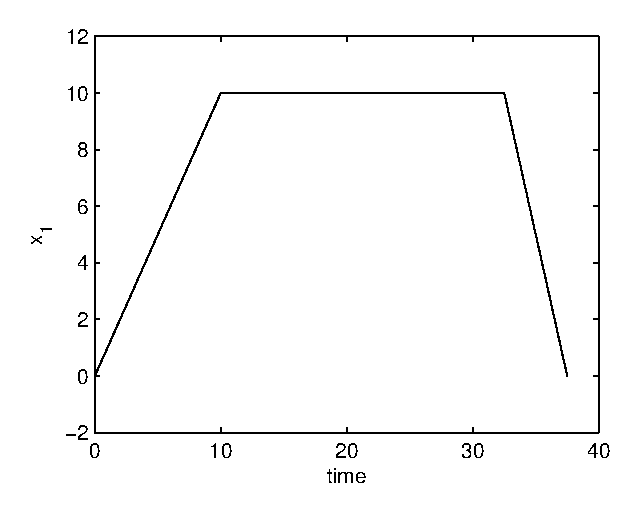
\includegraphics[width=0.32\textwidth]{examples/problem-car2/car_x1.eps}
\includegraphics[width=0.32\textwidth]{examples/problem-car2/car_x2.eps}
\caption{Control and state profiles for
  constrained minimum time car problem} \label{fig:car2} 
\end{figure}

\section{DAE systems}
\label{sec:daes}

\subsection{Example 6: Batch Reactor Problem}
\label{sec:brpdae}

Consider a batch reactor~\citep{raj01,dad95} with the 
consecutive reactions $A \rightarrow B\rightarrow C$ (MATLAB code for this example is located
at \subor{examples/problem5dae}):
\begin{equation}
\max_{\ve{u}(t)} \mf{J} = x_{2}(t_{f}) \label{eq:batch_dae}
\end{equation}
such that
\begin{gather}
\dot{x}_{1} = -k_{1}x_{1}^{2}, \qquad x_1(0) = 1 \\
\dot{x}_{2} = k_{1}x_{1}^{2} - k_{2}x_{2}, \qquad x_2(0) = 0 \\
0 = k_{1} - 4000e^{(-\frac{2500}{T})} \\
0 = k_{2} - 620000e^{(-\frac{5000}{T})} 
\end{gather} with $x_{1}, x_{2}$ as states representing concentrations
of A, and B, temperature $T \in [298,398]$ as control variable, such
that $t_{f} = 1$.

\subsubsection{Function~\fun{process},~\fun{objfun},~\fun{confun}  definitions}
\label{sec:example-fundef}

\paragraph{Step1: Write an M-file~\subor{process.m}}

{\small \verbatiminput{examples/problem5_dae/process.m}}

\paragraph{Step2: Write an M-file~\subor{objfun}}

{\small \verbatiminput{examples/problem5_dae/objfun.m}}

\paragraph{Step3: Invoke~\fun{dynopt}} by writing an
M-file~\subor{problem5dae.m} as follows:

{\small \verbatiminput{examples/problem5_dae/problem5.m}}

After 134 iterations, optimal value of $x_{2}(t_{f}) = 0.6106136$ was
found using fmincon. The same solution was found using ipopt but after
almost 20000 iterations. Graphical representation of the problem
\eqref{eq:batch_dae} solution is shown in Figs. \ref{fig:prob5dae_u}
and \ref{fig:prob5dae_x}.

\begin{figure}[htb]
\begin{minipage}[t]{0.5\linewidth}
\centering
\includegraphics[width=0.99\textwidth]{examples/problem5_dae/graphs/u_523daea.eps}
\caption[Tutorial example 6: control profile]{Control profile for
  batch reactor problem as DAE problem}\label{fig:prob5dae_u} 
\end{minipage}
\begin{minipage}[t]{0.5\linewidth}
\centering
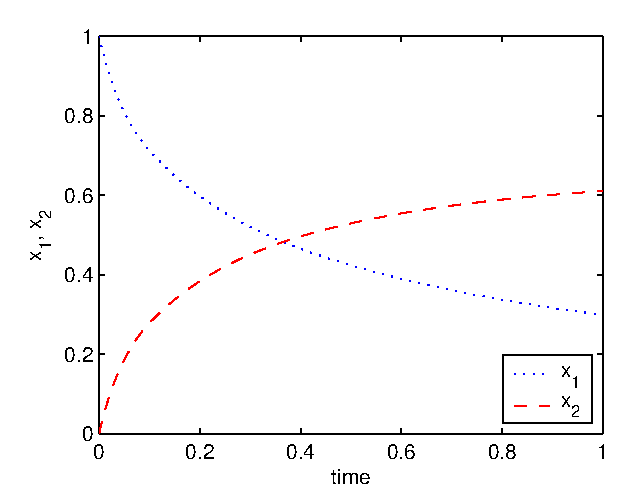
\includegraphics[width=0.99\textwidth]{examples/problem5_dae/graphs/x12_523daea.eps}
\caption[Tutorial example 6: state profiles]{State profiles for batch
  reactor problem as DAE problem}\label{fig:prob5dae_x} 
\end{minipage}
\end{figure}

\section{Maximisation}
\label{sec:maximisation}

\fun{dynopt} performs minimisation of the objective
function $f(t,x,u)$. Maximisation is achieved by supplying the
routine with $-f(t,x,u)$ . 

\section{Greater than Zero Constraints}
\label{sec:zeroconstraints}

The Optimisation Toolbox assumes nonlinear inequality constraints are
of the form $C_{i}(x)\leq 0$. Greater than zero constraints are
expressed as less than zero constraints by multiplying them by $-1$. For
example, a constraint of the form $C_{i}(x)\geq 0$ is equivalent to the
constraint $-C_{i}(x)\leq 0$. 



%%% Local Variables: 
%%% mode: latex
%%% TeX-master: "dynopt_guide"
%%% End: 
